
\begin{question}
In a deck of strange cards, each card has an image and a color. The
chance of drawing a gem is 45.1\%. If a gem is drawn, there is a 87\%
chance that it is red. If a card that is not a gem is drawn, there is a
21.5\% chance that it is red.

Now, someone draws a random card and reveals it is red. What is the
chance the card is not a gem?
\end{question}

\begin{solution}
I'd recommend making a tree. Remember, on the first branch, we put
simple probabilities. On the second branches we put conditional
probabilites. The results (products) are joint probabilities.

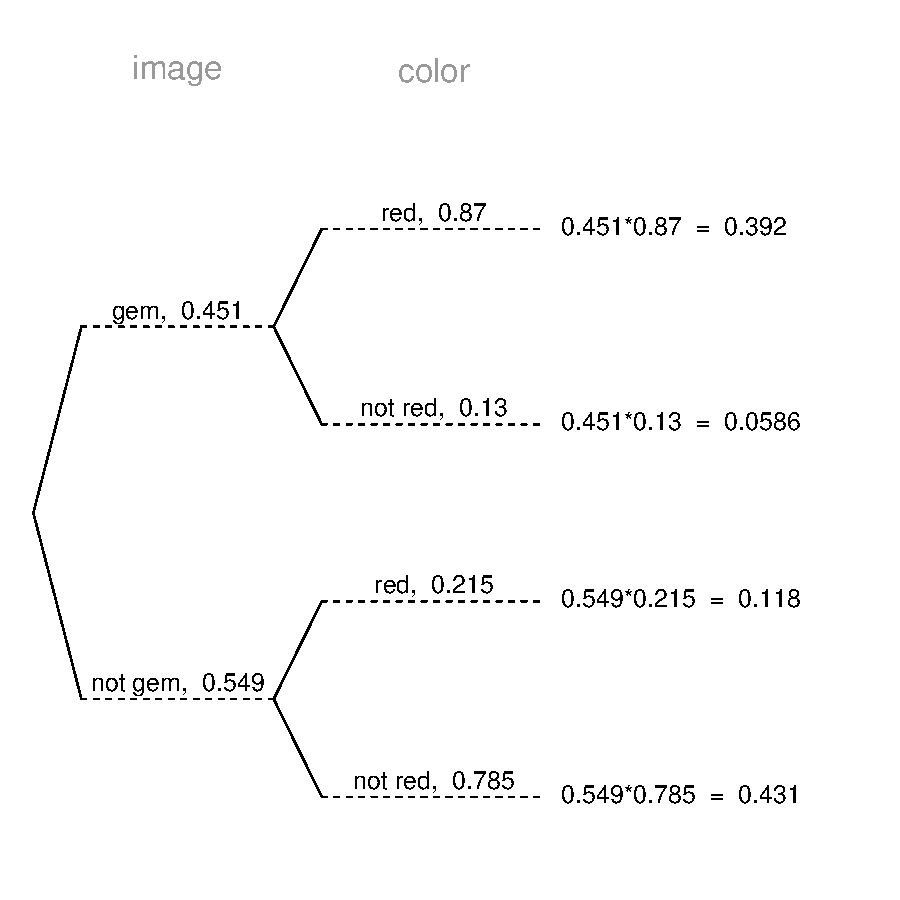
\includegraphics{tree-1.pdf} ~

Determine the appropriate conditional probability.
\[P(\text{"not gem" given "red"}) = \frac{0.118}{0.118+0.392} = 0.231 \]
\end{solution}

